\documentclass[pdftex,11pt,a4paper]{article}
\usepackage{anysize}
\marginsize{2.5cm}{2.5cm}{1.5cm}{1.5cm}
\usepackage[pdftex]{graphicx}
\usepackage{wrapfig}
\usepackage{url}
\usepackage{listings}
\usepackage{color}
\usepackage{textcomp}

\lstset{
	backgroundcolor=\color{lbcolor},
	tabsize=2,
	language=java,
	numbers=left,
	numbersep=5pt,
        basicstyle=\scriptsize,
        upquote=true,
        aboveskip={1.5\baselineskip},
        columns=fixed,
        showstringspaces=false,
        extendedchars=true,
        breaklines=true,
        prebreak = \raisebox{0ex}[0ex][0ex]{\ensuremath{\hookleftarrow}},
        showtabs=false,
        showspaces=false,
        showstringspaces=false,
        identifierstyle=\ttfamily,
        keywordstyle=\color[rgb]{0,0,1},
        commentstyle=\color[rgb]{0.133,0.545,0.133},
        stringstyle=\color[rgb]{0.627,0.126,0.941},
}



\definecolor{listinggray}{gray}{0.9}
\definecolor{lbcolor}{rgb}{0.9,0.9,0.9}
\linespread{1.2}
\setlength{\parindent}{0pt}
\setlength{\parskip}{1ex plus 0.8ex minus 0.2ex}

\usepackage{fancyhdr}

\pagestyle{fancy}
\lhead{\footnotesize {Systems Architecture Project} }
\rhead{\footnotesize {Client orders framework} }

\renewcommand\headheight{24pt}
\renewcommand\footrulewidth{0.4pt}

\clearpage
\newcommand{\HRule}{\rule{\linewidth}{0.5mm}}

\author{John \textsc{Flanagan} 0702009 \& Marcin \textsc{Wrzeszcz} 0726753 }
\title{TITLE GOES HERE}
\date{\today}

\begin{document}

\begin{titlepage}
 
\begin{center}
 
 
% Upper part of the page
%\includegraphics[width=0.8\textwidth]{images/logo.pdf}\\[3.5cm]
 
%\textsc{\LARGE Ubiquitous Merchant Legerity}\\[1.5cm]
 
\textsc{\LARGE Assignment 1}\\[3.5cm]
 
 
% Title
\HRule \\[0.6cm]
{ \huge \bfseries Retail software framework}\\Concurrent Architecture\\[0.4cm]
 
\HRule \\[4.0cm]
 {\large \today}\\[9.0cm]

\begin{flushleft} \large
\emph{Module:}\\
CS4135 Software Architecture
\\[0.4cm]
\emph{Authors:}\\
Marcin \textsc{Wrzeszcz} 0726753 \& John \textsc{Flanagan} 0702009
\end{flushleft}

 
\vfill
 

 
\end{center}
 
\end{titlepage}


\begin{center}
	Blank marking scheme
\end{center}

\pagebreak

\tableofcontents
\pagebreak

\section{Business scenario}
Our team have been tasked by a large computer manufacturer with the design and implementation of a software framework. They are attempting to automate their processes as well as hoping to sell products to customers online. The driver for their decision to automate  its processes has been predominately the current economic crisis, with them aiming to minimise administration staff with the introduction of this software. 

Like many of the large computer manufacturing corporations they have base products which the home or business user may customise to meet their requirements. The components that these products comprise of must be easily interchangeable. 

In the organisations drive to increase online sales, it is expected that this framework not only support integration with web services but also a number of unique business requirements. For example the framework should support support multiple regions taxes and currencies, composition rules for components and the simple addition of new base configurations and products.

While these requirements above may seem initially quite demanding, they are quite typical of the real world business demands for these types of framework.

\pagebreak
\section{Incorporated design patterns}
\subsection{Abstract factory}
\subsection{Factory method}
\subsection{State pattern}
\subsection{Builder pattern}
\subsection{Composite pattern}
\subsection{Observer pattern}

\pagebreak
\section{Creational design patterns}
In the scope of the framework we have two separate areas where creational design patterns are utilised, the creation of states for managing store locale and the creation of products. Of these the creation of products is the most interesting so we will concentrate on this primarily.

Our design for the generation of products aimed to keep the system as generic as possible, enabling developers to easily swap the ‘computer’ package with that of one which creates cars for example. With this requirement much consideration was given to its design and hierarchy. After much research and discussion we decided to use the abstract factory pattern in conjunction with the builder pattern. This enabled us to build factories for different products and for each factory control the assembly of each type of product.

Below is an simplification of our creational structure, in the outermost factory package only the most generic structures were defined, the ‘AbstractFactory’ and the ‘Product’ interface. Within the factory package a further package is created for category of product in this example these are the computer and printer packages.

\begin{center}
	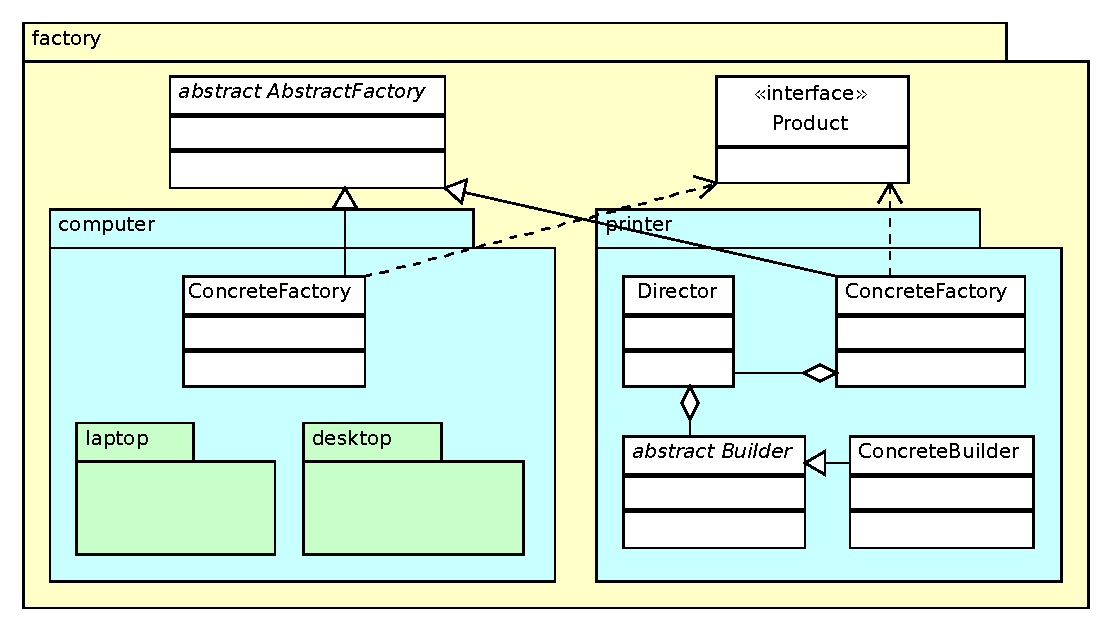
\includegraphics[scale=0.75]{images/creational_diagram.pdf}
\end{center}

This structure offered us the great flexibility in the creation of different product types, while maintaining ‘rules’ for the generation of each product type thanks to the inclusion of the builder pattern.

\subsection{Abstract factory}

To construct an implementation of the AbstractProductFactory you must pass the super type a reference to an observer, this enables us to register the \emph{OrderManager} as a observer of all products created. Which we in-turn use to notify the \emph{OrderManager} when a product is modified.

We designed the abstract factory to only have only one public interface \emph{createProduct(ProductsEnum)} which takes a \emph{ProductsEnum}. As ilustrated in the code fragment \emph{createProduct(ProductsEnum)} uses a switch statement to redirect the program flow to the relevant private method \emph{createGamingDesktopComputer()}. From these private methods we then instantiate a \emph{ComputerBuilder} which is really a director from the builder pattern and populate it with a \emph{ConcreteBuilder}.

This scheme enables us to in time add products of many types to the framework, while maintaining a level or rigidity among the product family's.

\lstinputlisting{code/abstractfactory.java}

\subsection{Builder pattern}

!!!!!how the builder works

\subsection{Observer in creation}
As previously mentioned when instantiating a factory we must pass a ‘OrderManager’ reference, we store this reference and on creation of a new product we register the ‘OrderManager’ as being an observer. This enables the order manager to perform a price recalculation every time a leaf is modified in the composite.

Although this implementation is not designed with performance in mind, as any time a composite is updated with a leaf we must rescan all products for a price change. This solution does offer a clean and structured way for ensuring we keep the cached price up-to-date in the \emph{OrderManager}.

\pagebreak

\section{Unit testing}

To create a reliable framework it is important to have good test coverage of the code, to ensure correctness firstly and secondly to help stop regressions being introduced to the framework. We chose to follow the Test-Driven Development paradigm, as it was a good indicator or development progress and also helped ensure a level of quality. This was largely a successful endeavour although on occasion it was easy to just continue working on the class without any test coverage and absolutely helped to drive the progress of development.

Our unit tests were created using the \emph{JUnit} testing framework\cite{website:junit}, the most common for the \emph{Java} platform. We found this to be quite easy to get up and running and the writing of tests was quite trivial.

\lstinputlisting{code/unittest.java}

In the above code sample, we have included an example of the type of test we are running against the framework. This particular test, performs a series of basic actions including adding a product and decorating a number of components. At the end we test that the price has increased, this test could be enhanced by calculating the extra price and ensuring the new price is equal to the old price plus the added components price.

Each of our tests contain a number of assertions, with any of which failing the overall test will fail. Outside of these individual tests we also use the \emph{setup()} method (not ilustrated here) to create a new instance of the \emph{OrderManager} for each test to ensure the preconditions are met.
\pagebreak


\section{Critique}
\subsection{Observer}
\emph{ComputerComposite}  is using observer whenever a change in composite occur i.e. new object is added,  removed or decorated. Every time this happens \emph{notifyObserver()} is invoked. Team's implementation of the observer pattern does not describe the nature of change that occured but only points to object that just changed.An improvement could be employed here -the method \emph{notifyObserver()} could return a reference to a leaf back to the observer. By using this improvement an observer could update its data via methods call on a leaf object. For example when user issues removal of a RAM, the RAM leaf instance would be dereferenced from its composite parent. Then the reference would be used by \emph{orderManager( RAM.getPrice() )} to update the \emph{totalPrice} value.
Currently \emph{orderManager} is notified that the state of \emph{computerProduct} has been altered, so it request \emph{getPrice()} on root element of \emph{computerProduct} and then it will execute this method on every node in tree to get \emph{totalPrice}.
If there are a lot of changes to \emph{computerProduct} then system would have to issue the \emph{getPrice()} method on it. This leads to costly and frequent reqursive calculation of total price. With improved implementation of the observer the \emph{orderManager} object needs to add/subtrack price value of received leaf from the total price.

\subsection{Composite Pattern: safe vs transparent}
Composite contains two lists, one for storing references to all composite children and second list for storing all leaves (components). If parent of composite class executes \emph{getChildern()}, composite class have to create a new list that contains "composites" and "leaves".
If \emph{getChildern()} call was to be executed repetevly then it might be a better idea to create a third list that contains other two lists. The overhead would be minimal as third list contais of references to already existing objects.
This is safe approach to design of the composite pattern as leves do not have access to the same methods as parent. It was found that it would be much easier to use transparent approach while designing composite. Transparent approach treats composite and leaf as the same object but leaf does not perform composite methods instead it contais stubs for those methods. So instead of two or three lists there would be only one needed as both composite and leaf are inheriting from the same interface/abstract class.

\subsection{UML workbench}
In this project team decided to use open source product to design all arcitectural diagrams - The Argo UML. However this tool was found to be at early stage of development and it lacks some esentila features, like undo functionality. Because of the UML workbench used by team that does not support the perfect and hundred  generation of class diagrams from the code the synchronisation of the UML model with the code would be too time consuming for the purpose of this project. Therfore at the stage in the project we were happy that we met the design pattern requirements. We used workbench to automaticaly generate the clasess and we chose not to keep model and the code in synch.

\subsection{Decorator}

Team discovered that implementation of the decorator patter could be achieved via two approaches. Wrapping the whole computer object with a decorator for example additional RAM, or particular composite object were to be wrapped with decorator i.e. RAM was wrapped with extra RAM. Even though the first approach was quickly decided to be easier approach it was found that it would decrease computer object flexibility after it was wrapped with additional decorators. Team decided that implementing decorators for each composite component would make code considerably more maintainable. Also accessing information about particular composite object through the computer object would be much easier to implement as there will not be any super class above computer that computer would have to know of.

\pagebreak

\section{Runtime Infrastructure/Technology Pipeline}
\subsection{Runtime/Colaboration Diagram}
This section contais a partial colaboration diagram of designed framework plus an abstrac client that uses framework. Due to system complexity and inferior colaboration diagram feature quality of UML workbench, the diagram was generalised and does not represent the whole system. But only flow of program related to adding and decorating a product.

\begin{center}
	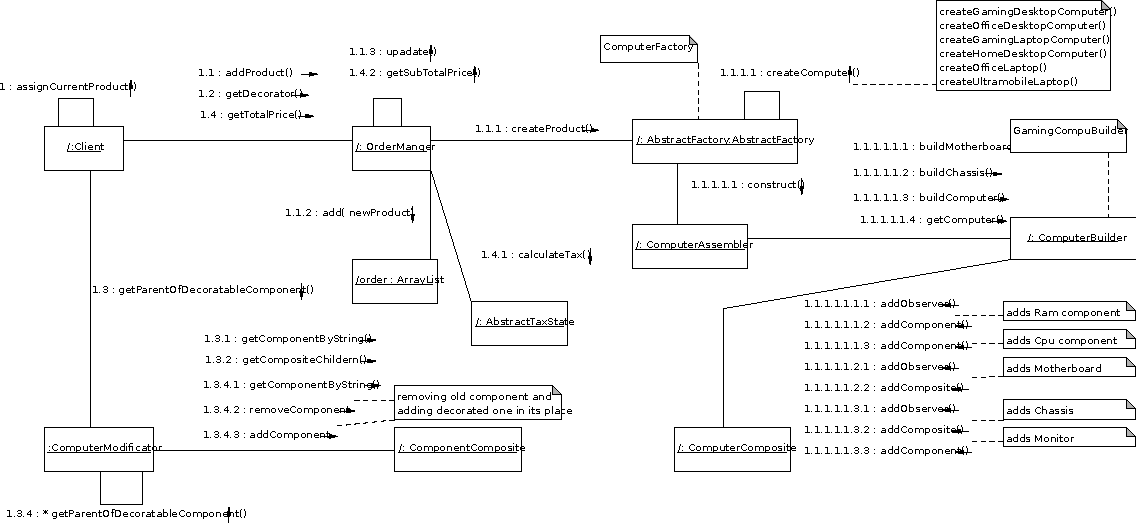
\includegraphics[scale=1, angle=90]{images/CollaborationDiagram.pdf}
\end{center}

\subsection{Architectural Use Cases}

\subsubsection{Computer Factory}
During the design phase team decided that \emph{ComputerFactory} class is going to contain following classes: \emph{createLowComputer()}, \emph{createMidComputer()}, \emph{createHighComputer()} and similar for creating all laptop products. However every time new produc would be added or old product would be changed it would require many major code rewrites in client's implementation. That is why it was decided to implement class \emph{createComputer(Enum type)} that would be responsible for creating a new instance of any computer (it contains : \emph{createLowComputer(}), \emph{createMidComputer()} and so on methods). Now client doesn't have to call each method separately instead it calls the same function with different parameter. This solution created a level of abstraction between client and factories and made code more reusable.

\subsubsection{Scalability and Reusability}
There are several cases in the UML diagram produced by the team of interfaces that look redundant (\emph{ComponentInterface}, \emph{DecoratorInterface}). They are either empty or are realised only by another interface which make them look redundant and unneccessary. However this was done on purpose to employ idea of reusability and scalability. Decorator interface might serve as interface to any product type, so it is not only tied to computer products. If in future a company decides to increase range of products that they want to distribute it would be easier for team to realise \emph{DecoratorInterface}, rather then refractor the code to support new range of products. 

\subsection{Code Selection}
Team found out that usage of strings as parameter for selecting products would be problematic and could create hard to read and hard to maintain code. Adding or removing product would be time consuming. The solution that team came up with was found to solve all problems - the usage of enumerations. Enumerations were used instead of strings for any method that was taking an parameter that was used as a way of selecting specific code, for example \emph{calculateTax(Enum region)} would execute only code responsible for calculating tax in particular region. This proved to be a very effective and robust way to deal with selection of code; furthermore switch case could be utilised with great readability improvement:

\lstinputlisting{code/ifAndOnlyIf.java}

Above inplementation of selection of one of three blocks of code using string. In terms of readability this code is average, but can be refacored into clean looking code as follows:

\lstinputlisting{code/switchCaseExample.java}

\pagebreak

\section{Deployment considerations}
Due to the inherently generic nature of the framework it is possible to be deployed on a number of infrastructures. As proof of concept we built both a traditional GUI application and a Representational State Transfer (RESTful)\cite{REST} implementation to utilise the framework. Representing the traditional and more modern sides of client/server architecture.

\subsection{Desktop application}

Graphical User Interface (GUI) was developed by the team as POC. GUI client was tied to framework's exposed (pulbic) methods. This was an alternative to web-services as GUI has direct access to framework and does not need any layers between client and framework. Even thought GUI is static application running on top of framework, it could be used to create a Desktop Application that would connect to framework's web services in future, if company requests it.

\subsubsection{Vendor offerings}
Java's swing library was first and most obvious candidate as tool for building GUI. It is very well documented and powerful library. Second option was to use  Python GTK library. PyGTK applications like Java are multiplatform and they're able to run, unmodified, on Linux, Windows, MacOS X and other platforms.
Besides its ease of use and rapid prototyping, its first class accesibility support or the capability to deal with complex multilingual or bidirectional text for fully localized applications. However team discovered that it can be quite time consuming to design GUI and then tie it to Java framework.
NetBeans GUI builder was found to suit team needs, as it has powerful features combined with intuative interface. Then the dummy user Interface was connected to the underlaying framework

\subsubsection{Development issues}
Initialy team was looking for Eclipse GUI builder plugin, but due to difficulties with instalation of Visual Editor, team turned to NetBeans GUI builder. This posed some difficulties. User interface was designed in NetBeans and then code was copied into Eclipse enviroment. Whenever team decided to change or adjust the GUI it involved manual code changes. This turned out to be quite time consumming. All team members agreed that in future only tools within team's IDE of choice would be use, as they save time in long time by solving problems of `translating' code between different IDEs.
Because Java swing builds threaded applications team run into a problem of accessing resources of one window from another (one thread of another). As design of GUI involved 'Control Window and 'Add Product Window', when user presses Add product from 'Control Window' it will pop-up 'Add Product Window' where user can select a product that can be added to list of products. This is why 'Add Product Window' needs to have a reference to its parent so that can add a product to parent's orderManager list.

\subsection{Webservice}

Web-services are a popular mechanism for exposing a software's functionally over HTTP with a high degree of system and language interoperability. These services can be broadly categorised into RPC and Resource based.

RPC (remote procedure call) is a tried and tested mechanism, and is conceptually an extension to a regular or local procedure call. But due to this constraint of exposing a specific function, these mechanisms tended to be quite system and language dependant. In 2000 Roy Fielding presented his doctoral dissertation where he described "Representational State Transfer"\cite{REST} which described a mechanism modeled around the standard HTTP (GET, POST, UPDATE, DELETE) operations and were resource orientated (giving each entity a unique URI) as opposed to the RPC stored state paradigm. RESTful services have be steadily gaining momentum, and due to this popularity and language/system abstraction, we chose to create a RESTful web-service as a proof of concept for the framework.

\subsubsection{Vendor offerings}
Because of the simplicity of the REST concept, which is based on HTTP which has only four operations as mentioned earlier. There are frameworks for creating RESTful applications for almost every conceivable language, from Clojure\cite{website:compojure-rest} to Javascript\cite{website:persevere}. It is common for developers to use a REST framework that runs within a Application Server such as Tomcat\cite{website:tomcat} or JBoss\cite{website:jboss}. But due to the lightweight nature of the paradigm we were keen on not running the service on a heavy weight application server.

A number of light weight REST frameworks for Java exist, below are a list of the more popular offerings.

\begin{itemize}
	\item \textbf{JAX-RS} A Java JCP spec for RESTful webservices utilising Java Annotations. A number of implementations of the specification exist Apache CXF, Jersey, RESTEasy and Restlet.
	\item \textbf{Zipwire-REST} A framework based on the ActiveResource pattern which enables Java object to be manipulated through REST, is a lightweight manner.
	\item \textbf{SerfJ}
\end{itemize}

\subsubsection{Restlet}
Restlet was chosen for this development as it seemed to be the most modern of the feature complete and lightweight frameworks. Restlet also conforms to the JAX-RS JCP specification\cite{website:jax-rs_jcp} making the knowledge gained from this endeavour more valuable.

This library is available under a number of different licences including CDDL ver 1.0, LGPL ver 2.1, LGPL ver 3.0 and EPL ver 1.0. Some larger companies may have difficulty with these licences due to the lack of freedom licences like BSD or Apache offer.

The popularity of this framework is evident in the number of maintained ports for platforms such as Google Web Toolkit, Google App Engine and Android as well as versions for both Java EE and Java SE.

\begin{center}
	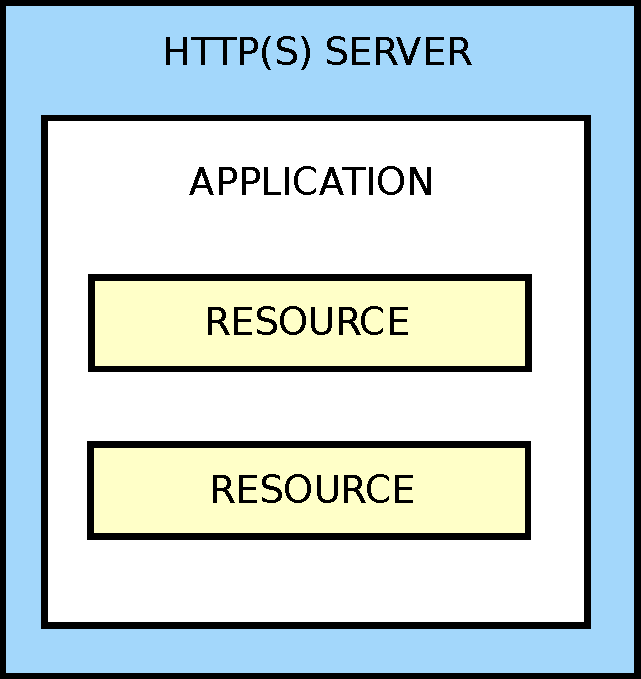
\includegraphics[scale=0.5]{images/restlet_structure.pdf}
\end{center}

The Restlet structure is quite simple the hierarchy consists of Server, Application and a  Resource. The HTTP server is contained in the library, enabling the developer to build and deploy the project without any extra software.  The value in this feature is with slight modification the developer can re-package the service for a Application Server.

\lstinputlisting{code/OrderResource.java}

Each of the resources ilustrated in the diagram above have a unique URL \\ e.g. \emph{http://server/application/resource1}.

\subsubsection{Development issues}

\paragraph{JSON or XML}
A RESTful service can be developed to communicate any form of data, but the two most commonly used today are XML and JSON. JSON (Javascript object notation) is a lightweight data representation which Javascript uses to store its data. Using JSON not only enables better usage of bandwidth but also enables the front-end developer to easily consume data from your web-service. Below is an example of a JSON object.

\lstinputlisting{code/json.js}

\paragraph{Object serialization}
Difficulties arose when attempting to convert the \emph{OrderManager} object in to its JSON representation, due to a number of reasons. Firstly the existences of circular references in the object model, these make it very difficult for a serialize to walk the dependency tree. Secondly the use of decorated components in the composite can become quite unwieldy when converted to their JSON representation.

As a quick ’n dirty hack we created a separate JSON representation for the \emph{OrderManager}, containing all the data required by a client. Because of this we needed to maintain state on the server side (something which runs against REST architectural pattern), so the server held a reference to that \emph{OrderManager} for a specific client.
With a little refactoring of the \emph{OrderManager}, we believe it is possible to use it in a correctly RESTful implementation.

\paragraph{Web browser security model}
During implementation of the web-service we used the Mozilla FireFox plug-in REST Client\cite{website:restClient} to ensure correctness of the service. Later when beginning to implement a Javascript based front-end we began to run into troubles with the browser security model.

All modern web browsers have security restrictions on the execution of GET, POST, UPDATE and DELETE HTTP methods, when the executing code was not served from that domain. This is a really important security mechanism which prevents a script on domainx.com from downloading your emails from freemail.com.

It is possible to enable these HTTP methods for scripts from other domains, and its is necessary for a number of reasions, including serving your site content from js.myservice.com and having the REST endpoints on rest.myservice.com. This is enabled by setting a HTTP content header parameter in the responses from the REST endpoint.  Two specific headers define the rules for these transactions \emph{Access-Control-Allow-Origin} and \emph{Access-Control-Allow-Methods}, below is an example of headers with the access enabled.

\begin{center}
	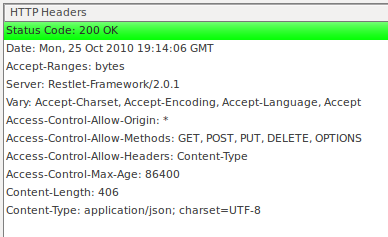
\includegraphics[scale=.7]{images/content_headers.png}
\end{center}

This only became an issue as we were running Restlet with its inbuilt web server, which did not enable us to host files on the same domain (domain and port). Java based rest services are typically hosted in a Application Server environment and this does not become an issue, because all the files are packaged in the WAR (web application achieve) enabling the content to be hosted with the resources.

\paragraph{Browser issues}
Due to this slightly unusual configuration we got bogged down with an issue in both Mozila Firefox and Google Chrome. In developing the front end, I began by using the Dojo toolkit (Javascript framework)\cite{website:dojo}, watching the server output noticed it was calling the service with the HTTP OPTIONS instead of HTTP GET. After some time researching the problem (believed to be related to requesting data from another domain), it was suggested using a Javascript raw \emph{XMLHTTPRequest} call which worked for a GET request, but unfortunately I was unable to get it working for a POST request again sending a OPTIONS request. 

We are not sure how to proceed with the Javascript client application without moving to an Application Server.


\pagebreak

\section{UML Diagrams}


\pagebreak


\def\refname{}
\bibliography{references}
\bibliographystyle{plain}

\end{document}
